\chapter{Inbetriebnahme} \label{cha:inbetriebnahme}

\section{Einführung}

In diesem Kapitel werden die Maßnahmen für das Deployment der Anwendung näher beschrieben. Anhand einer Übersicht wird gezeigt, wie das System im laufenden Zustand aussieht und wie die unterschiedlichen Anwendungen mit unserem Backend interagieren.

\section{Backend Containerisierung}

\begin{figure}[H]
  \centering
  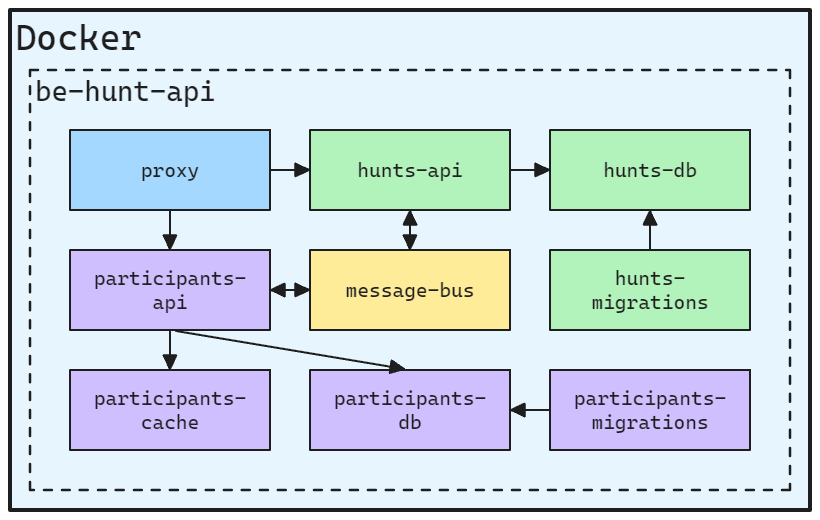
\includegraphics[width=\textwidth]{images/PrAr_Depl_Docker.png}
  \caption{UML-Diagramm für das Deployment}
  \label{fig:deployment:docker}
\end{figure}

Abbildung \ref{fig:deployment:docker} stellt die Deployment-Ansicht des Backends dar. Das Deployment wird durch die Docker Containerisierung ermöglicht (vgl. Kapitel \ref{cha:grundlagen:swtech:docker}). Die Konfiguration der verschiedenen Dienste wird über eine \textit{Docker-Compose} Datei definiert.

Der Proxy (vgl. Abbildung \ref{fig:deployment:docker} - blau) fungiert als zentraler Einstiegspunkt für die Anwendungen von außen. Er leitet alle Anfragen an den jeweils richtigen Dienst weiter. Bei falschen oder ungültigen Anfragen bricht die Verbindung ab. Die Implementierung und Konfiguration des Proxies ist im Anhang beschrieben.

Die beiden Container Participants-Api und Hunts-Api (vgl. Abbildung \ref{fig:deployment:docker} - grün und violett) sind die deployten Release-Builds der entworfenen Services aus Kapitel \ref{cha:swentwurf:backend}. Diese haben jeweils eigene Datenbank-Container für die Persistierung von Daten.

Für die initiale Erstellung und Aktualisierung bestehender Datenbank-Container sind zusätzlich die beiden Migration-Container \textit{Participants-Migrations} und \textit{Hunts-Migrations} vorgesehen (vgl. Abbildung \ref{fig:deployment:docker} - grün und violett). Beide öffnen eine Verbindung zur jeweiligen Datenbank und erstellen die initial benötigten Datenbanktabellen, damit diese für die Verwendung im jeweiligen Service mit den aktuellen Datenbanktabellen existieren.

Die jeweiligen Dockerfiles sind im Anhang näher beschrieben (vgl. Anhang \ref{appendix:code:dockercompose}).

\section{Frontend Containerisierung}

Da das Frontend mit Web-Technologien (vgl. Kapitel \ref{cha:grundlagen:swtech:svelte}) implementiert wurde, kann es als plattformunabhängige Browseranwendung auf einem Webserver deployt werden. Dies ist auch über Docker Containerisierung möglich, wurde aber im Rahmen des Projektes nicht entworfen und getestet.

Für das Deployment der Hunt-Editor Web-App für Desktops wäre es auch möglich, eine echte Anwendung daraus zu machen. Hierfür stehen bereits implementierte Technologien wie \textit{Tauri} zur Verfügung (siehe \autocite{github:tauri} und \autocite{tauri:tauri}).
